\chapter{An\'alisis de requisitos y dise\~no}\label{requisitos}

\section{Participantes del proyecto}

\bigskip

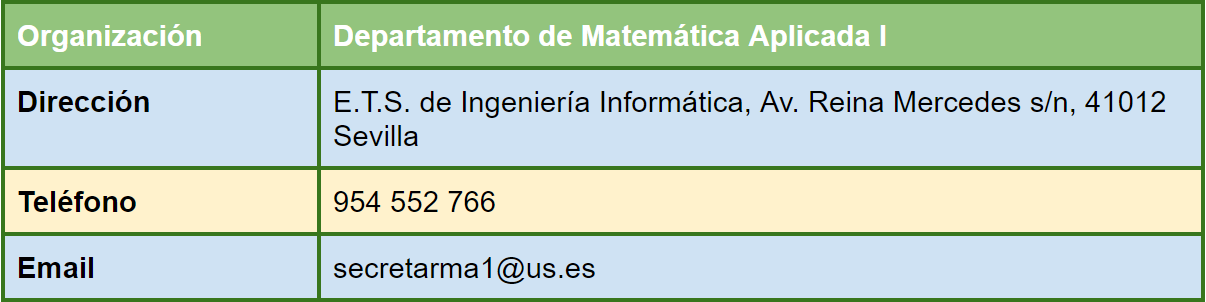
\includegraphics[width=\textwidth]{img/cap5/participantes/1.png}

\bigskip

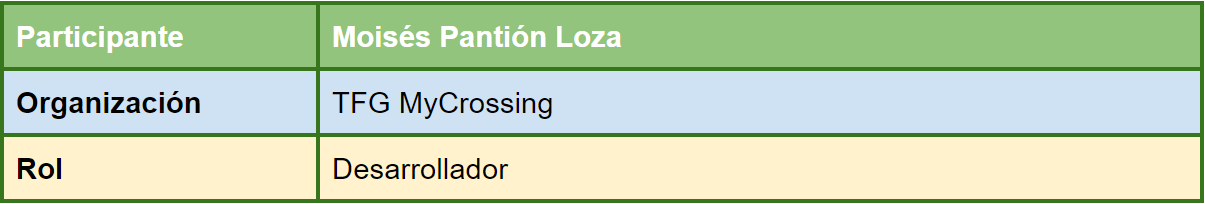
\includegraphics[width=\textwidth]{img/cap5/participantes/2.png}

\bigskip

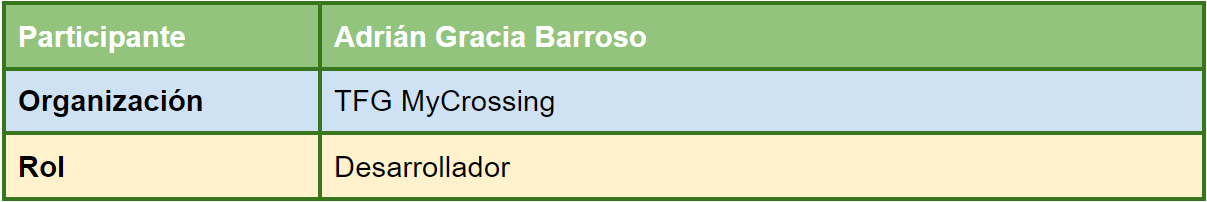
\includegraphics[width=\textwidth]{img/cap5/participantes/3.png}

\bigskip

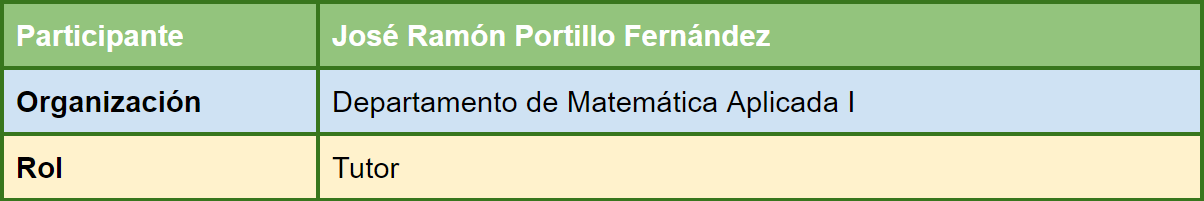
\includegraphics[width=\textwidth]{img/cap5/participantes/4.png}

\bigskip

\section{Requisitos}
	\subsection{Requisitos de Informaci\'on}
	
	\bigskip
	
	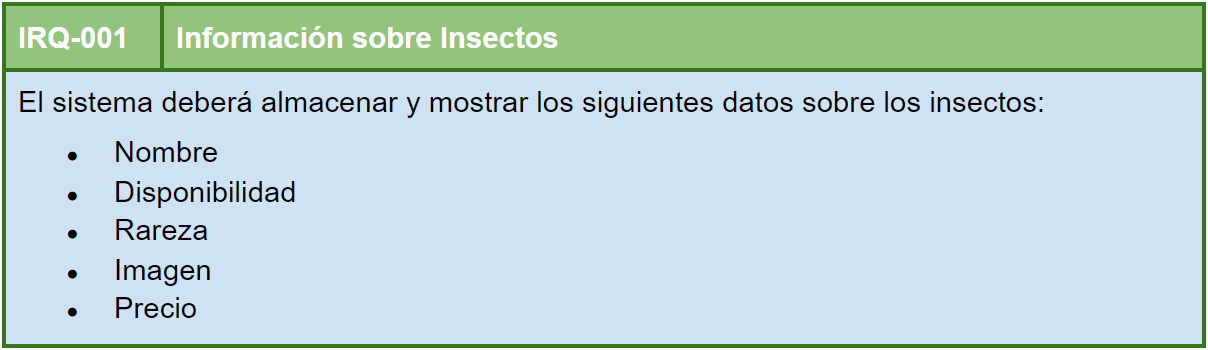
\includegraphics[width=\textwidth]{img/cap5/IR/1.png}
	
	\bigskip
	
	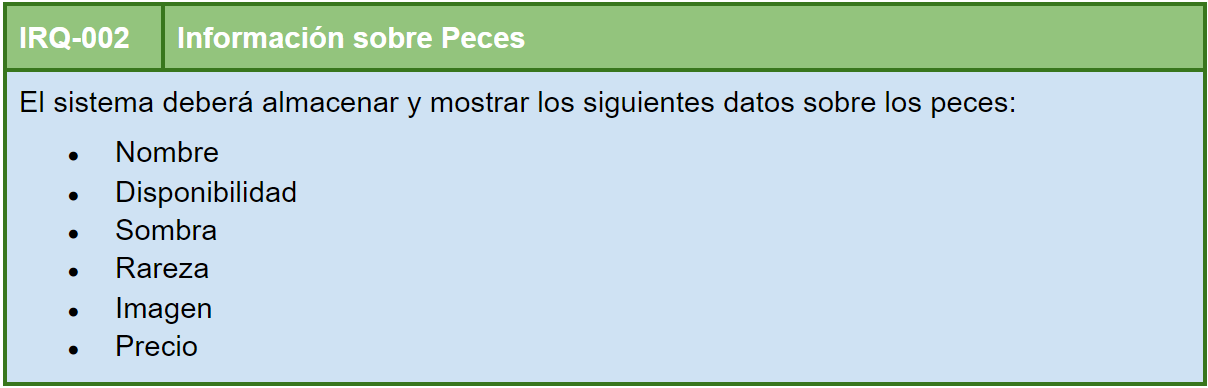
\includegraphics[width=\textwidth]{img/cap5/IR/2.png}
	
	\bigskip
	
	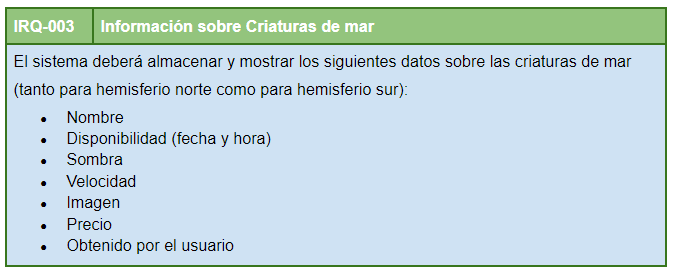
\includegraphics[width=\textwidth]{img/cap5/IR/3.png}
	
	\bigskip
	
	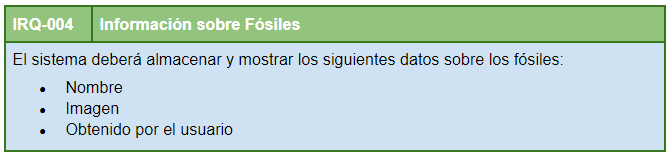
\includegraphics[width=\textwidth]{img/cap5/IR/4.png}
	
	\bigskip
	
	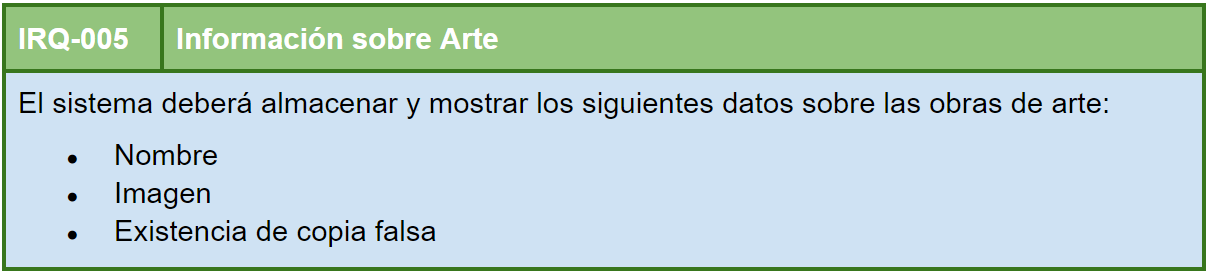
\includegraphics[width=\textwidth]{img/cap5/IR/5.png}
	
	\bigskip
	
	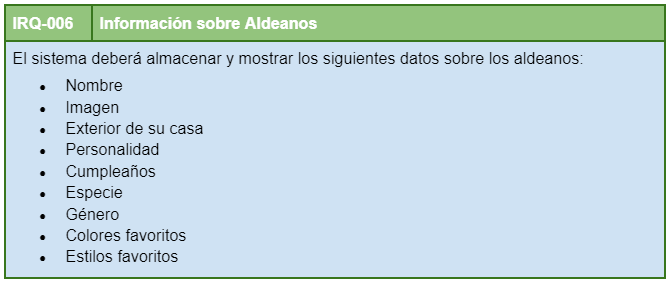
\includegraphics[width=\textwidth]{img/cap5/IR/6.png}
	
	\bigskip
	
	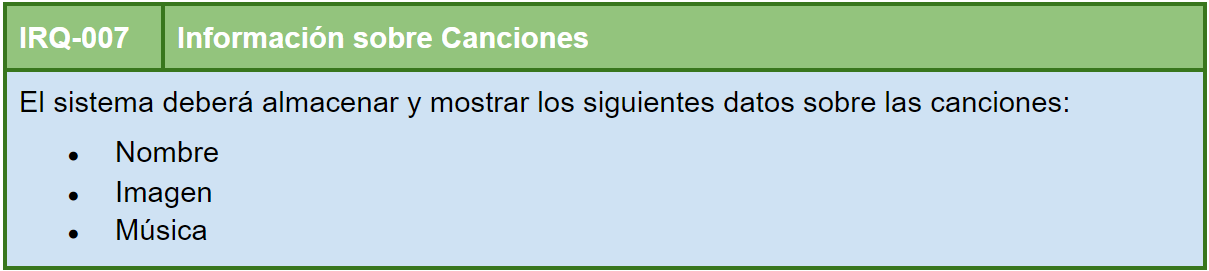
\includegraphics[width=\textwidth]{img/cap5/IR/7.png}
	
	\bigskip
	
	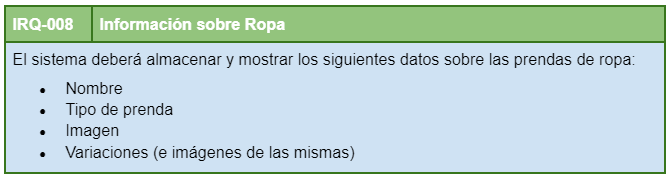
\includegraphics[width=\textwidth]{img/cap5/IR/8.png}
	
	\bigskip
	
	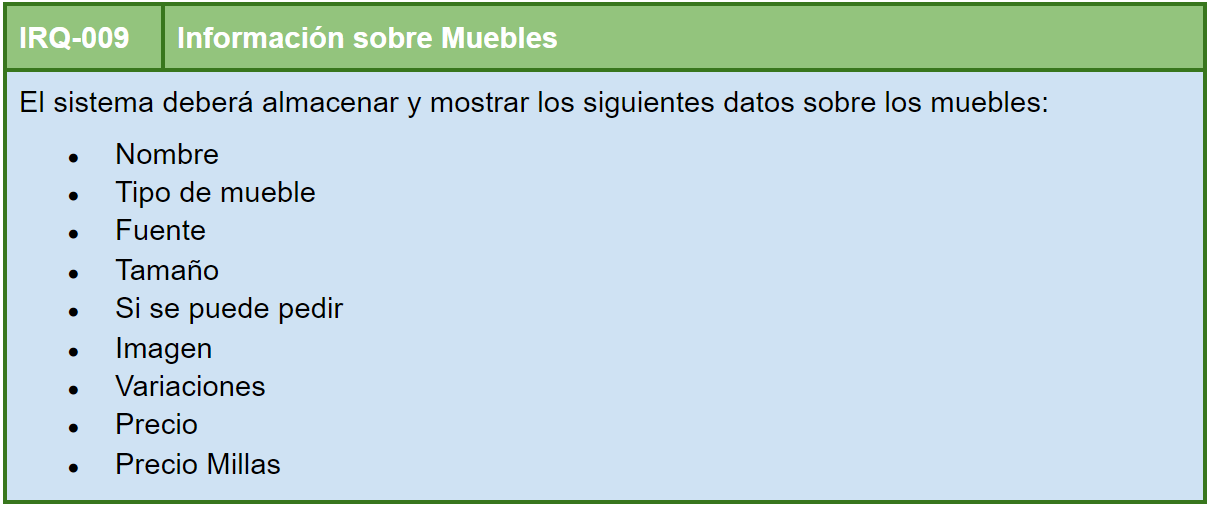
\includegraphics[width=\textwidth]{img/cap5/IR/9.png}
	
	\bigskip
	
	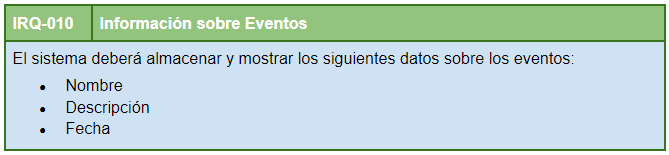
\includegraphics[width=\textwidth]{img/cap5/IR/10.png}
		
	\subsection{Requisitos Funcionales}
	
	\bigskip
	
	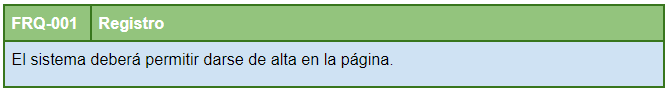
\includegraphics[width=\textwidth]{img/cap5/FR/1.png}
	
	\bigskip
	
	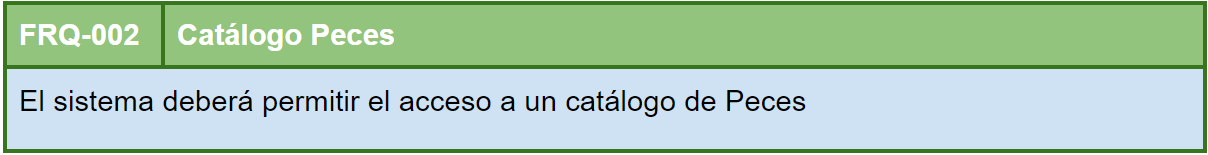
\includegraphics[width=\textwidth]{img/cap5/FR/2.png}
	
	\bigskip
	
	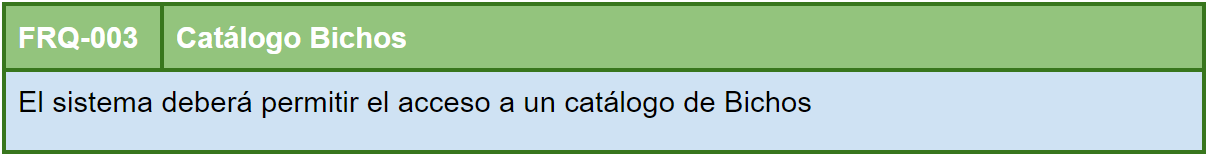
\includegraphics[width=\textwidth]{img/cap5/FR/3.png}
	
	\bigskip
	
	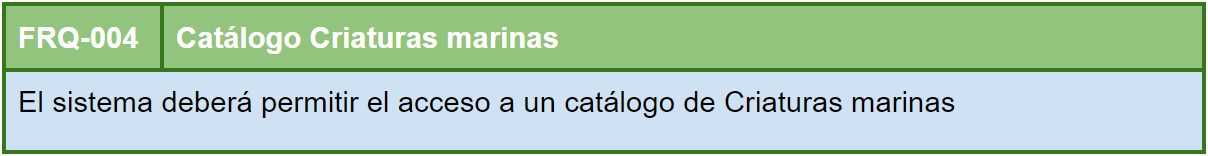
\includegraphics[width=\textwidth]{img/cap5/FR/4.png}
	
	\bigskip
	
	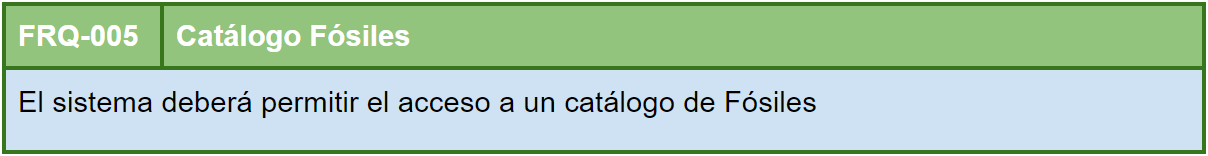
\includegraphics[width=\textwidth]{img/cap5/FR/5.png}
	
	\bigskip
	
	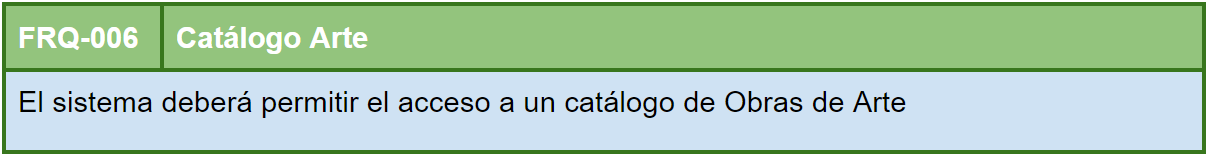
\includegraphics[width=\textwidth]{img/cap5/FR/6.png}
	
	\bigskip
	
	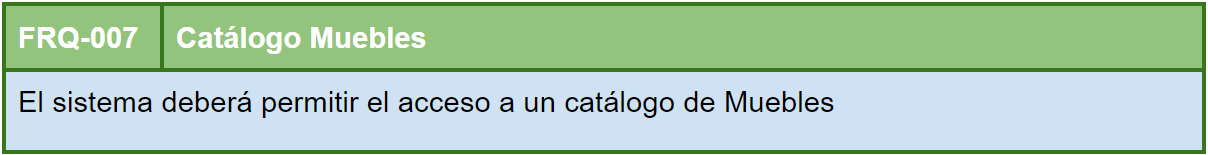
\includegraphics[width=\textwidth]{img/cap5/FR/7.png}
	
	\bigskip
	
	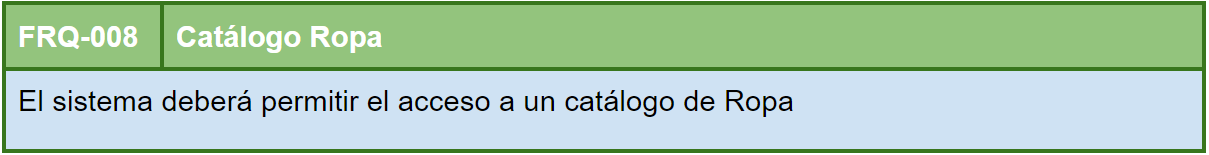
\includegraphics[width=\textwidth]{img/cap5/FR/8.png}
	
	\bigskip
	
	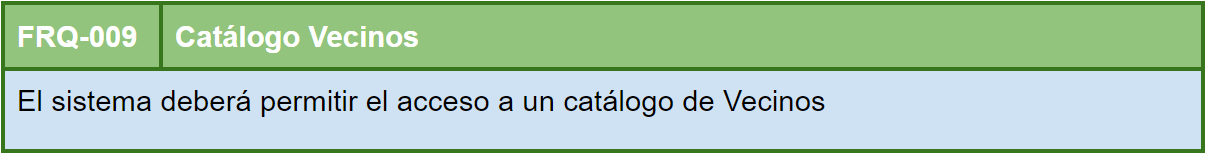
\includegraphics[width=\textwidth]{img/cap5/FR/9.png}
	
	\bigskip
	
	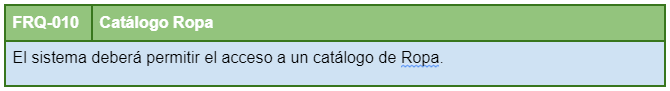
\includegraphics[width=\textwidth]{img/cap5/FR/10.png}
	
	\bigskip
	
	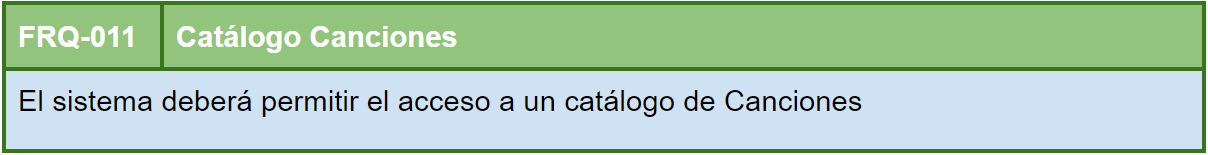
\includegraphics[width=\textwidth]{img/cap5/FR/11.png}
	
	\bigskip
	
	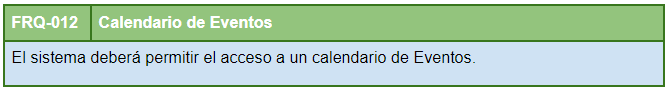
\includegraphics[width=\textwidth]{img/cap5/FR/12.png}
	
	\bigskip
	
	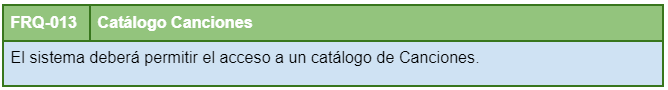
\includegraphics[width=\textwidth]{img/cap5/FR/13.png}
	
	\bigskip
	
	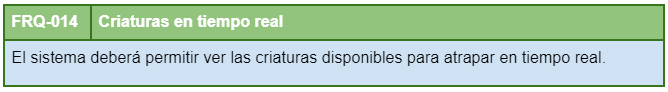
\includegraphics[width=\textwidth]{img/cap5/FR/14.png}
	
	\bigskip
	
	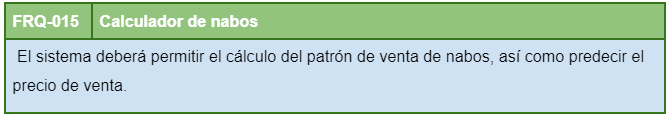
\includegraphics[width=\textwidth]{img/cap5/FR/15.png}
	
	\bigskip
	
	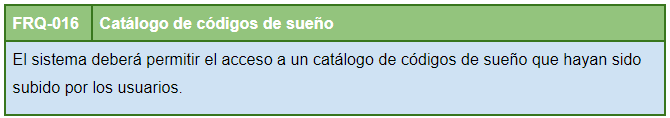
\includegraphics[width=\textwidth]{img/cap5/FR/16.png}
	
	\bigskip
	
	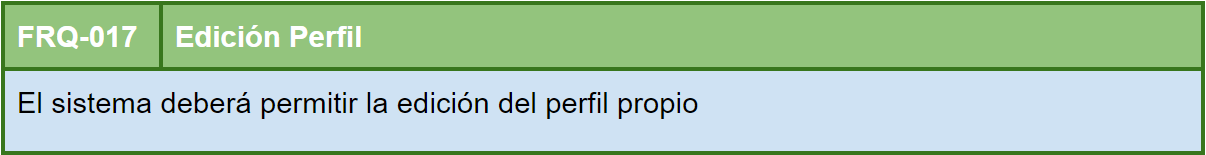
\includegraphics[width=\textwidth]{img/cap5/FR/17.png}
	
	\bigskip
	
	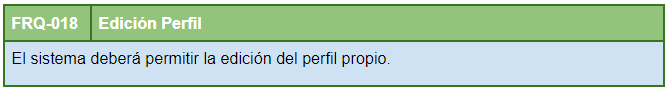
\includegraphics[width=\textwidth]{img/cap5/FR/18.png}
	
	\bigskip
	
	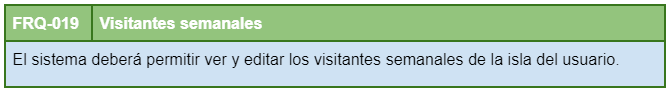
\includegraphics[width=\textwidth]{img/cap5/FR/19.png}
	
	\bigskip
	
	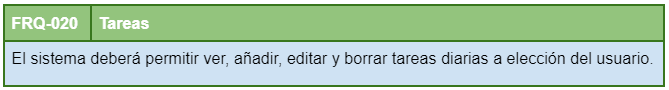
\includegraphics[width=\textwidth]{img/cap5/FR/20.png}
	
	\bigskip
	
	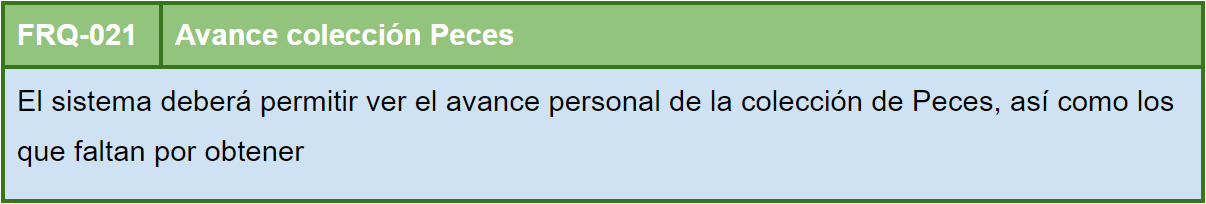
\includegraphics[width=\textwidth]{img/cap5/FR/21.png}
	
	\bigskip
	
	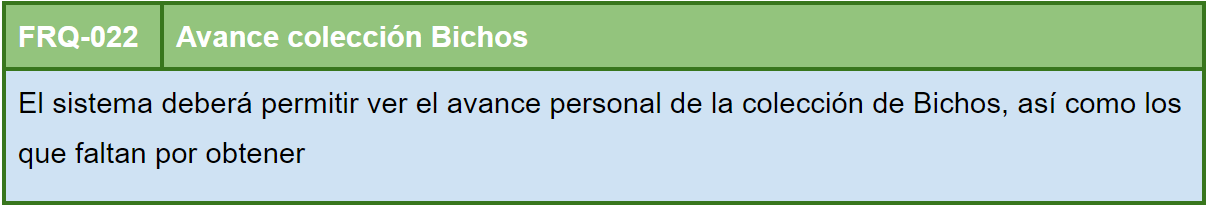
\includegraphics[width=\textwidth]{img/cap5/FR/22.png}
	
	\bigskip
	
	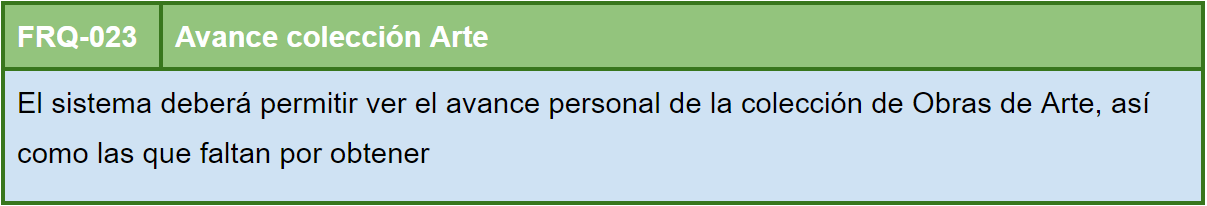
\includegraphics[width=\textwidth]{img/cap5/FR/23.png}
	
	\bigskip
	
	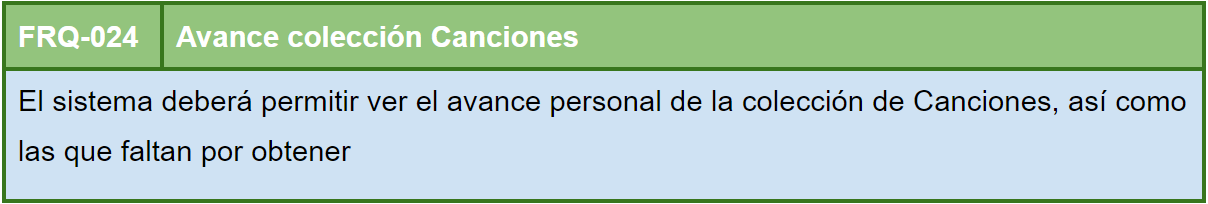
\includegraphics[width=\textwidth]{img/cap5/FR/24.png}
	
	\bigskip
	
	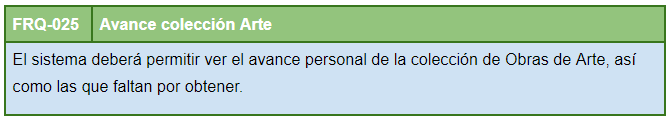
\includegraphics[width=\textwidth]{img/cap5/FR/25.png}
	
	\bigskip
	
	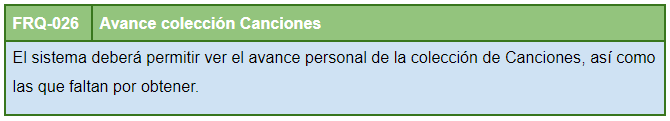
\includegraphics[width=\textwidth]{img/cap5/FR/26.png}
	
	\bigskip
	
	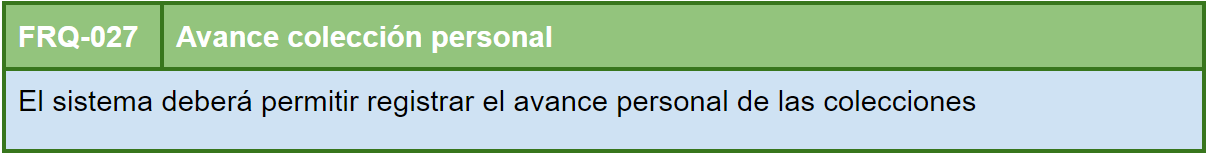
\includegraphics[width=\textwidth]{img/cap5/FR/27.png}
	
	\bigskip
	
	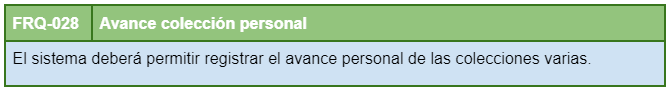
\includegraphics[width=\textwidth]{img/cap5/FR/28.png}
	
	\bigskip
	
	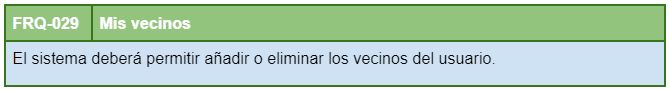
\includegraphics[width=\textwidth]{img/cap5/FR/29.png}
	
	\bigskip
	
	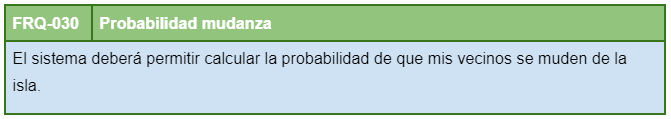
\includegraphics[width=\textwidth]{img/cap5/FR/30.png}

	\subsection{Requisitos no Funcionales}
	
	\bigskip
	
	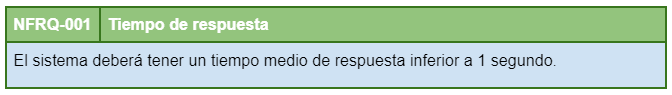
\includegraphics[width=\textwidth]{img/cap5/NFR/1.png}
	
	\bigskip
	
	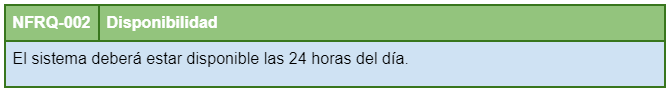
\includegraphics[width=\textwidth]{img/cap5/NFR/2.png}
	
	\clearpage
	
\section{Diagrama de Clases}

	A continuación podemos ver un esquema a de alto nivel de las relaciones de las entidades de la aplicación, así como la información que contiene cada objeto. Dado que tratamos con grandes cantidades de información, gran parte de ella la tenemos que obtener a través de APIs.\\
	
	Debido al gran tamaño del diagrama de clases, vamos a verla dividida en partes más pequeñas de forma que muestren distintas relaciones y se pueda ver de forma más clara.\\
	
		\bigskip
	
	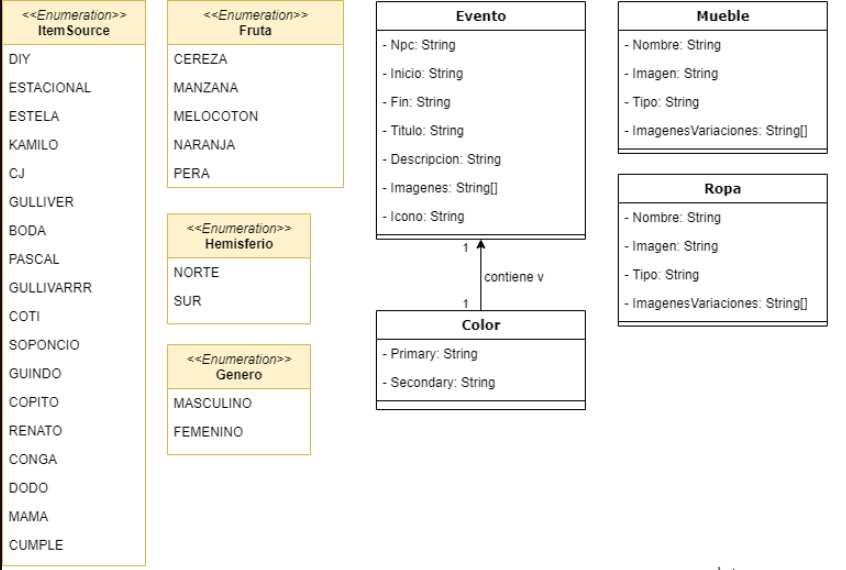
\includegraphics[width=\textwidth]{img/cap5/diagramaclases/enum-y-no-relacionados.png}
	
		\bigskip
	
	Primero podemos ver tanto los enumerados, como algunas clases que se encuentran más aisladas, ya que no forman parte del gran conjunto que rodea al usuario y por lo tanto, son datos puramente informativos y no se almacenará en base de datos. En este caso se trata de los muebles y las prendas de ropa (que como vemos, son idénticos), así como los eventos, que están relacionados con la clase Color, pero nada más lejos de dicha relación.\\ 
	
	\clearpage
	
	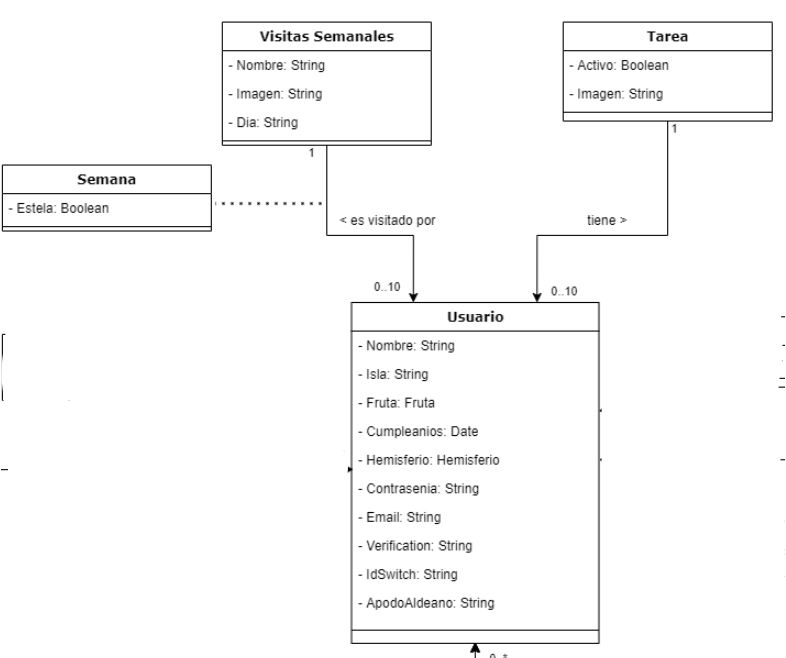
\includegraphics[width=\textwidth]{img/cap5/diagramaclases/tareas-visitas.png}
	
		\bigskip
	
	Pasando al conjunto principal, podemos empezar por la relación que comparte la clase Usuario con Visitas y Tareas. Un Usuario puede tener de 0 a 10 Tareas, al igual que pasa con Vistas Semanales, aunque esta tiene además una relación con usuario que indica si Estela (un personaje del juego) ha visitado ya la isla o no.\\
	
		\bigskip
	
	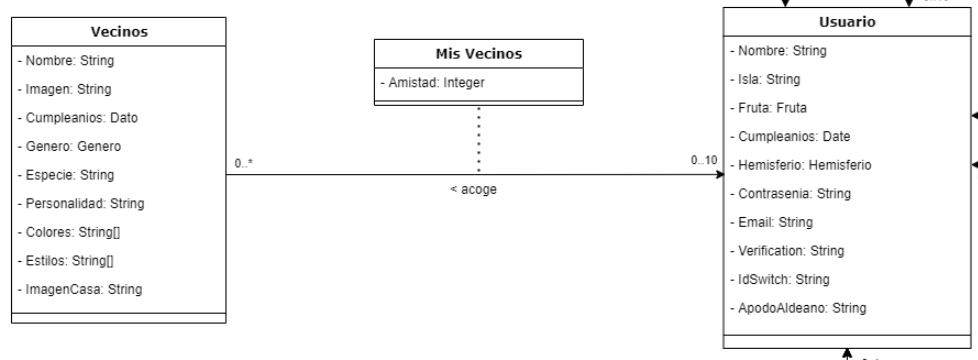
\includegraphics[width=\textwidth]{img/cap5/diagramaclases/vecinos.png}
	
		\bigskip
	
	Luego, podemos ver la relación de Vecinos que, al mostrarse tanto en un catálogo (en el cual no se registra la relación con el usuario), como en el perfil (donde sí se opera y registra con dicha relación), vemos que tiene una relación Mis Vecinos que relaciona aquellos Vecinos que estén habitando en la isla del Usuario, además con el atributo Amistad para indicar la amistad que tiene cada uno con el jugador.\\
	
	\clearpage
	
	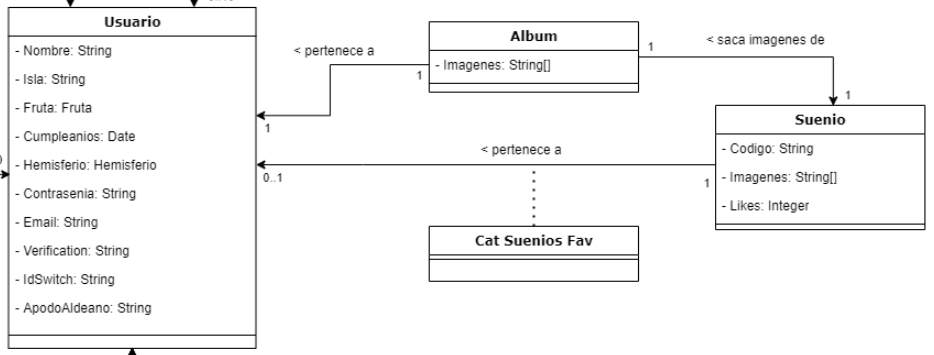
\includegraphics[width=\textwidth]{img/cap5/diagramaclases/suenios.png}
	
		\bigskip
	
	Seguimos con la relación de Usuario con Sueños. Esta entidad esta relacionada a su vez con Álbum, que también está relacionada con Usuario. Un Usuario dispone de un Álbum de fotos, las cuales se pueden utilizar para añadir imágenes al sueño de dicho Usuario. Además, un Usuario puede tener un listado de Sueños a los que le haya dado "Me Gusta".\\ 
	
		\bigskip
	
	\includegraphics[width=\textwidth]{img/cap5/diagramaclases/catalogos.png}
	
		\bigskip
	
	Por último, tenemos una serie de listados que se relacionan todos de la misma manera con Usuario (la punta de la flecha superior). Cada entidad tiene su propia página de listado, y cada Usuario dispone de un catálogo personal de cada entidad en el cual se añaden aquellas entidades que ya haya obtenido.\\
	
	\clearpage
	
	Para terminar, se incluye una imagen completa del diagrama de clases para tener una vista global del mismo.\\
	
		\bigskip
	
	\includegraphics[width=\textwidth]{img/cap5/diagramaclases/diagrama-completo.png}
	
\clearpage

\section{Dise\~no}

A continuación ofrecemos una primera visión de lo que sería la interfaz gráfica del sistema, acompañado de algunas explicaciones para entender a priori el funcionamiento  del sistema, ya que entraremos en detalle más adelante en el manual de usuario. En las imágenes aparecen anotaciones realizadas en rojo para el mejor entendimiento del estilo que se busca obtener de cara a la hora de implementar las vistas.\\

Empezando por la página de inicio (v\'ease la figura~\ref{fig:inicio1}), tendríamos el navegador en la zona superior para acceder a las diferentes secciones del sistema que no necesitan que el usuario se haya registrado, además de un botón para iniciar sesión en caso de que se disponga de una cuenta en la página.\\

\begin{figure}[!htb]
	\begin{minipage}{0.48\textwidth}
		\centering
		\includegraphics[width=\linewidth]{img/mockups/Inicio - 1.png}
		\caption{Inicio 1}
		\label{fig:inicio1}
	\end{minipage}\hfill
	\begin{minipage}{0.48\textwidth}
		\centering
		\includegraphics[width=\linewidth]{img/mockups/Inicio - 2.png}
		\caption{Inicio 2}
		\label{fig:inicio2}
	\end{minipage}
\end{figure}

Bajando vemos diferentes secciones, disponiendo en primer plano de la portada con un botón para acceder al registro. Más abajo se encuentran las diferentes secciones de enciclopedia con las que contará el sistema: peces, bichos, criaturas marinas, fósiles y obras de arte , así como del catálogo de muebles, ropa, vecinos e incluso un calendario de eventos {(v\'ease la figura~\ref{fig:inicio2})}.\\

\clearpage

Empezando por las secciones que hemos comentado en el párrafo anterior, a continuación tenemos un listado de peces, aunque el formato es genérico para los demás listados, cambiando algunos pequeños detalles en cada uno como ciertos filtros.\\

Podemos observar que arriba se encuentra la sección de filtros para que el usuario pueda realizar una búsqueda más específica de manera simple. Debajo de los filtros se encuentra el listado en sí, que muestra una recopilación de los peces (en este caso) disponibles en el juego. Cada ítem cuenta con una imagen, su nombre y algunos de los datos más relevantes, como precio de venta o localización, y si se hace clic en la celda se abre un menú con información más detallada, de forma que lo importante esté siempre a la vista y no haya que entrar en los menús de forma repetitiva.\\
 
En rojo se muestran aquellas criaturas que no se encontrarán disponibles el mes que viene, y además, si el usuario está registrado en el sistema y ha iniciado sesión, puede llevar recuento de los que ya ha capturado marcándolos con el tick superior derecho en cada ítem, cambiándose así el fondo a un color distinto para diferenciarlos a simple vista {(v\'ease la figura~\ref{fig:listado})}.\\

\figura{1}{img/mockups/Listado.png}{Listado genérico}{fig:listado}{}

\clearpage

Para terminar con el contenido de la página de inicio (ya que a excepción del calendario, lo demás son todo listados como el que acabamos de ver), tendríamos el calendario de eventos {(v\'ease la figura~\ref{fig:eventos1})}.\\

\figura{0.7}{img/mockups/Eventos - 1.png}{Eventos}{fig:eventos1}{}

Esta sección no es mas que un gran calendario donde el usuario puede ver tanto las festividades del juego como los cumpleaños de los vecinos. Sin embargo, dispondrá de información adicional para los eventos al hacer clic en ellos, de forma que se desplegará un menú {(v\'ease la figura~\ref{fig:eventos2})} en el que podremos ver información útil de dicho evento, como visitantes, objetos temáticos, actividades especiales, etc. De esta forma el usuario puede tener una idea general de todo lo que se puede hacer en ese evento y planificarse mejor su agenda.\\

\figura{0.8}{img/mockups/Eventos - 2.png}{Eventos - Detallado}{fig:eventos2}{}

\clearpage

Una vez acabado con el contenido de la página principal, si el usuario quisiera registrarse accedería a la siguiente vista {(v\'ease la figura~\ref{fig:mockregistro})}, la cual es una simple página de registro con información relevante al juego, como el nombre de la Isla, el tipo de fruta o la localización. Este último es bastante importante ya que dependiendo de si se encuentra en el hemisferio norte o sur, el usuario visualizará unos datos u otros.\\

\figura{1}{img/mockups/Registro.png}{Registro}{fig:mockregistro}{}

Si se completa el registro de forma satisfactoria, se puede acceder al perfil del usuario, el cual dispone de varias secciones {(v\'ease la figura~\ref{fig:mockperfil})}.\\

\figura{0.8}{img/mockups/Perfil.png}{Perfil}{fig:mockperfil}{}

A la izquierda se muestra la información del usuario a modo de resumen o biografía. A la derecha se encuentra la sección que se usará de forma diaria. Por una parte tenemos las tareas, las cuales se pueden editar con un icono dependiendo del propósito que tengan y serán marcadas por el usuario una vez hayan sido realizadas, reiniciándose cada día. Por otra parte tenemos la lista de visitantes semanales, donde podremos observar los visitantes de la semana anterior e ir rellenando los de esta semana en consecuencia.\\

Si bajamos, encontraremos un listado de los vecinos que actualmente residen en nuestra isla, con posibilidad de ir añadiendo hasta un máximo de diez vecinos. Al colocar el cursor sobre cualquiera de ellos, se mostrará información sobre el mismo.\\

Más abajo tenemos un pequeño listado de algunas colecciones de objetos especiales para que el usuario lleve un recuento de las que ya dispone y las pueda localizar de una manera más sencilla y organizada. Las colecciones irán variando dependiendo de que botón se encuentre activo, y dispondrá de un recuadro de texto para realizar una búsqueda específica.\\

Por último, tenemos una sección de galería que sirva a modo de portfolio para el usuario, para tener todas las capturas y/o vídeos recopilados en un mismo sitio.\\

\clearpage

Una vez acabado con el perfil, pasamos a las tres últimas vistas que se encuentran en el navegador principal de la página. Primero encontramos una página que es una recopilación de listados (como el mencionado anteriormente) de bichos, peces y criaturas marinas. La diferencia, aparte de encontrarse los tres juntos, es que en este listado aparecen todas las criaturas que se pueden atrapar actualmente, actualizándose a medida que lo hace el tiempo {(v\'ease la figura~\ref{fig:cazarahora1})}. Esto es útil ya que si un usuario quiere saber que criaturas puede cazar ahora en su isla, tan solo tiene que acceder a esta página y ya dispone de dicha información, sin registro ni pérdida de tiempo, ya que dispone de las tres colecciones de criaturas en la misma página.\\

Además, también dispone de una serie de filtros para realizar una búsqueda algo más específica, incluso con opciones de ocultar cierta información para evitarse así los "spoilers", de forma que sepa donde puede encontrar la criatura pero no sepa ni cuál ni cómo es, de esta forma puede tener una cierta ayuda a la hora de capturarla pero seguir teniendo la emoción de no saber que es lo que le aguarda.\\

\begin{figure}[!htb]
	\begin{minipage}{0.48\textwidth}
		\centering
		\includegraphics[width=\linewidth]{img/mockups/Cazar Ahora - 1.png}
		\caption{Cazar ahora 1}
		\label{fig:cazarahora1}
	\end{minipage}\hfill
	\begin{minipage}{0.48\textwidth}
		\centering
		\includegraphics[width=\linewidth]{img/mockups/Cazar Ahora - 2.png}
		\caption{Cazar ahora 2}
		\label{fig:cazarahora2}
	\end{minipage}
\end{figure}

\clearpage

A continuación tendríamos la calculadora de nabos. En esta página se proporciona un poco de información acerca del mercado de nabos dentro del juego, de forma que el usuario entienda algo mejor como funciona y los distintos patrones de venta que existen {(v\'ease la figura~\ref{fig:nabos})}.\\

En la parte inferior se encontraría la calculadora en sí, donde el usuario debe de escribir la información que haya ido recopilando para poder así realizar una predicción del patrón que hay actualmente en su isla. Además se acompañará de una gráfica y una tabla de precios por si quisiera información más detallada.\\

\figura{1}{img/mockups/Nabos.png}{Calculadora de Nabos}{fig:nabos}{}

\clearpage

Para terminar con este apartado y con el capítulo, por último veremos la vista del probador. Esta es una de las funcionalidades que crearemos y que consiste, como su propio nombre indica, en un probador de ropa {(v\'ease la figura~\ref{fig:probador})}.\\

En el centro tendremos una imagen de nuestro personaje, al cual podremos personalizar utilizando el menú superior, actualizándose a medida que seleccionemos las distintas opciones. Una vez elegido el personaje, la página dispondrá de un catálogo de ropa dividido en secciones (cabeza, torso, accesorios etc) para que el usuario pueda buscar la prenda que quiera probarse. Una vez la encuentre, con un clic sobre la prenda, esta aparecerá sobre el personaje central. Además se mostrarán en un desplegable todas las variaciones de color de las prendas para obtener así un catálogo completo. De esta forma el usuario puede realizar combinaciones de ropa para probar nuevos estilos y decidir que prendas necesita, en vez de ir comprándolas en el juego para luego cambiar de opinión.\\

\figura{0.9}{img/mockups/Probador.png}{Probador}{fig:probador}{}